% This is text associated with the open textbook "Open Electromagnetics"
% See immediately below for author, date
% <License info goes here (boilerplate, not read by project compiler)>

%ORB TITLE Phasors
%ORB AUTHOR 0        # S.W. Ellingson, Virginia Tech (ellingson@vt.edu)
%ORB DATE 20180814   # yyyymmdd
%ORB ABSTRACT Phasors: Basic concepts, conversion to and from time-domain, properties, comments on applicability

\label{m0033_Phasors} % <-- Must match name of this file and module directory name.  Don't mess with this!
\index{phasor|(}

In many areas of engineering, signals are well-modeled as sinusoids.
Also, devices that process these signals are often well-modeled as linear time-invariant (LTI) systems.
The response of an LTI system to any linear combination of sinusoids is another linear combination of sinusoids having the same frequencies.\footnote{ A ``linear combination'' of functions $f_i(t)$ where $i=1,2,3,...$ is $\sum_i {a_i f_i(t)}$ where the $a_i$'s are constants.}
In other words, 
(1) sinusoidal signals processed by LTI systems remain sinusoids and are not somehow transformed into square waves or some other waveform; and 
(2) we may calculate the response of the system for one sinusoid at a time, and then add the results to find the response of the system when multiple sinusoids are applied simultaneously.
This property of LTI systems is known as \emph{superposition}.
\index{superposition}

The analysis of systems that process sinusoidal waveforms is greatly simplified when the sinusoids are represented as \emph{phasors}.
Here is the key idea:
%
%ORB HIGHLIGHT
\begin{mdframed}[backgroundcolor=yellow!20,nobreak=true] 
A \emph{phasor} 
\index{phasor (definition)}
is a complex-valued number that represents a real-valued sinusoidal waveform.  Specifically, a phasor has the magnitude and phase of the sinusoid it represents.
\end{mdframed}

Figures~\ref{m0033_fComplexPlane} and \ref{m0033_fSinusoids} show some examples of phasors and the associated sinusoids.  
%
\begin{figure}
\begin{center}
\pdftooltip{{  % note double braces
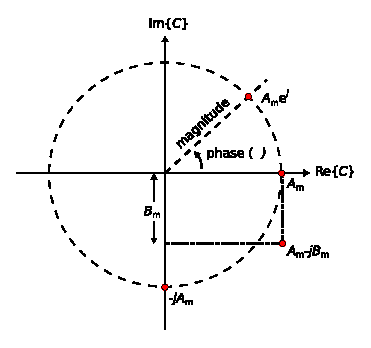
\includegraphics[width=3in]{modules/m0033_fComplexPlane.eps}
}}{A dotted circle is plotted on an imaginary versus real plane with the origin as its center. A rectangle is superimposed on the plane with vertices at (0, 0), (0, -j B sub m), (A sub m, 0) and (A sub m, -j B sub m)  B sub m is the distance along the negative imaginary axis. A sub m is the distance along the positive real axis and is equal to the radius of the circle. In the positive real quadrant, magnitude is labeled as an line running from the origin to the circle at a phase angle of psi. The magnitude line intersects at the point A sub m * e raised to the quantity i * psi.}
\end{center} 
%\vspace{3in}
\caption{\label{m0033_fComplexPlane} Examples of phasors, displayed here as points in the real-imaginary plane.
}
\end{figure}
%
\begin{figure}
\begin{center}
\pdftooltip{{  % note double braces
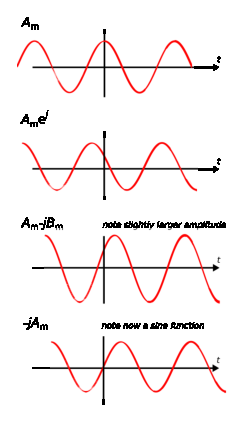
\includegraphics[width=2.5in]{modules/m0033_fSinusoids.eps}
}}{The figure shows four graphs in a column, each featuring sinusoidal waves with the x-axis labeled t. The top is labeled A sub m, and the middle wave, maximum amplitude intersects on the y-axis. The second is labeled A sub m * e raised to the quantity of j psi, and the middle wave maximum amplitude is slightly to the left of the y-axis. The third is labeled A sub m * quantity of -j B sub m, and has a slightly larger amplitude than the first or second with the middle wave maximum amplitude slightly to the right. The fourth is labeled -j * A sub m, and the midpoint intersects the origin.}
\end{center} 
\caption{\label{m0033_fSinusoids} Sinusoids corresponding to the phasors shown in Figure~\ref{m0033_fComplexPlane}.}
\end{figure}

It is important to note that a phasor by itself is not the signal.  
A phasor is merely a simplified mathematical representation in which the actual, real-valued physical signal is represented as a complex-valued constant. 

Here is a completely general form for a physical (hence, real-valued) quantity varying sinusoidally with angular frequency $\omega=2\pi f$:
%
\begin{equation}
A(t;\omega) = A_m(\omega) \cos{(\omega t + \psi(\omega))}
\end{equation} 
%
where 
$A_m(\omega)$ is magnitude at the specified frequency, 
$\psi(\omega)$ is phase at the specified frequency, 
and $t$ is time.  
Also, we require $\partial A_m/\partial t =0$; that is, that the time variation of $A(t)$ is completely represented by the cosine function alone. 
Now we can equivalently express $A(t;\omega)$ as a phasor $C(\omega)$:
%
\begin{equation}
C(\omega) = A_m(\omega) e^{j\psi(\omega)}
\label{m0033_eCOmega}
\end{equation}
%
To convert this phasor back to the physical signal it represents, we (1) restore the time dependence by multiplying by $e^{j\omega t}$, and then (2) take the real part of the result.  In mathematical notation: 
%
%ORB HIGHLIGHT
\begin{mdframed}[backgroundcolor=yellow!20,nobreak=true] 
\begin{equation}
A(t;\omega) = \mbox{R{e}} \left\{ C(\omega) e^{j\omega t} \right\}
\label{m0033_ePhasor}
\end{equation} 
\end{mdframed}
%
To see why this works, simply substitute the right hand side of Equation~\ref{m0033_eCOmega} into Equation~\ref{m0033_ePhasor}.  Then:
\begin{equation}
\begin{split}
A(t) & = \mbox{Re}\left\{ A_m(\omega) e^{j\psi(\omega)} e^{j\omega t} \right\} \\
    ~& = \mbox{Re}\left\{ A_m(\omega) e^{j\left(\omega t + \psi(\omega)\right)} \right\} \\
    ~& = \mbox{Re}\left\{ A_m(\omega) \left[   \cos\left(\omega t + \psi(\omega)\right)  \right. \right. \\
    ~& ~~~~~~~~~~~~~~~ \left.              \left. +j\sin\left(\omega t + \psi(\omega)\right)  \right] \right\} \\
    ~& = A_m(\omega) \cos\left(\omega t + \psi(\omega)\right) 
\end{split}
\nonumber
\end{equation}
%
as expected.

It is common to write Equation~\ref{m0033_eCOmega} as follows, dropping the explicit indication of frequency dependence:
%
\begin{equation}
C = A_m e^{j\psi}
\end{equation}
%
This does not normally cause any confusion since the definition of a phasor requires that values of $C$ and $\psi$ are those that apply at whatever frequency is represented by the suppressed sinusoidal dependence $e^{j\omega t}$.   

Table~\ref{m0033_tPhasorExamples} shows mathematical representations of the same phasors demonstrated in Figure~\ref{m0033_fComplexPlane} (and their associated sinusoidal waveforms in Figure~\ref{m0033_fSinusoids}).
It is a good exercise is to confirm each row in the table, transforming from left to right and vice-versa.
%
\begin{table*}[t]
\begin{center}
\begin{tabular}{ll|l}
$A(t)$ & ~ & $C$ \\
\hline
$A_m \cos \left( \omega t \right)$ & ~ & $A_m$ \\
$A_m \cos \left( \omega t + \psi \right)$ & ~ & $A_m e^{j\psi}$ \\  
$A_m \sin \left( \omega t \right)$ & $= A_m \cos \left( \omega t - \frac{\pi}{2}\right)$ & $-jA_m$ \\  
$A_m \cos \left( \omega t \right) + B_m \sin \left( \omega t \right)$ & $= A_m \cos \left( \omega t \right) + B_m \cos \left( \omega t - \frac{\pi}{2}\right)$ & $A_m-jB_m$ \\  
\end{tabular}
\end{center}
\caption{\label{m0033_tPhasorExamples}Some examples of physical (real-valued) sinusoidal signals and the corresponding phasors. $A_m$ and $B_m$ are real-valued and constant with respect to $t$. 
}
\end{table*}

It is not necessary to use a phasor to represent a sinusoidal signal.  
We choose to do so because phasor representation leads to dramatic simplifications.
For example:
%  
\begin{itemize}
\item Calculation of the peak value from data representing $A(t;\omega)$ requires a time-domain search over one period of the sinusoid. However, if you know $C$, the peak value of $A(t)$ is simply $\left|C\right|$, and no search is required.
\item Calculation of $\psi$ from data representing $A(t;\omega)$ requires correlation (essentially, integration) over one period of the sinusoid. However, if you know $C$, then $\psi$ is simply the phase of $C$, and no integration is required.
\end{itemize}
%
Furthermore, mathematical operations applied to $A(t;\omega)$ can be equivalently performed as operations on $C$, and the latter are typically much easier than the former. 
To demonstrate this, we first make two important claims and show that they are true.

\rule{3in}{1pt}\\~\\

{\bf Claim 1}: Let $C_1$ and $C_2$ be two complex-valued constants (independent of $t$).  Also,  $\mbox{Re} \left\{ C_1 e^{j\omega t} \right\} = \mbox{Re} \left\{ C_2 e^{j\omega t} \right\}$ for all $t$.  Then, $C_1=C_2$. 

{\it Proof:} Evaluating at $t=0$ we find $\mbox{Re} \left\{ C_1 \right\} = \mbox{Re} \left\{ C_2 \right\}$.  Since $C_1$ and $C_2$ are constant with respect to time, this must be true for all $t$.  At $t=\pi/(2\omega)$ we find
%
\begin{equation}
\mbox{R{e}} \left\{ C_1 e^{j\omega t} \right\} = \mbox{R{e}} \left\{ C_1 \cdot j \right\} = -\mbox{Im} \left\{ C_1 \right\}
\nonumber
\end{equation}
%
and similarly
%
\begin{equation}
\mbox{R{e}} \left\{ C_2 e^{j\omega t} \right\} = \mbox{R{e}} \left\{ C_2 \cdot j \right\} = -\mbox{Im} \left\{ C_2 \right\}
\nonumber
\end{equation}
%
therefore $\mbox{Im} \left\{ C_1 \right\} = \mbox{Im} \left\{ C_2 \right\}$. Once again: Since $C_1$ and $C_2$ are constant with respect to time, this must be true for all $t$.  Since the real and imaginary parts of $C_1$ and $C_2$ are equal, $C_1 = C_2$. 

{\it What does this mean?} We have just shown that if two phasors are equal, then the sinusoidal waveforms that they represent are also equal. 

\rule{3in}{1pt}\\~\\

{\bf Claim 2}:  For any real-valued linear operator $\mathcal{T}$ and complex-valued quantity $C$, $\mathcal{T}( \mbox{Re}\left\{ C \right\} ) = \mbox{Re}\left\{ \mathcal{T}(C) \right\}$.

{\it Proof:} Let $C = c_r + jc_i$ where $c_r$ and $c_i$ are real-valued quantities, and evaluate the right side of the equation:
%
\begin{equation}
\begin{split}
\mbox{Re}\left\{ \mathcal{T}(C) \right\}& = \mbox{Re}\left\{ \mathcal{T}(c_r + jc_i) \right\} \\
                                       ~& = \mbox{Re}\left\{ \mathcal{T}(c_r) + j\mathcal{T}(c_i) \right\} \\
                                       ~& = \mathcal{T}(c_r) \\
                                       ~& = \mathcal{T}( \mbox{Re}\left\{ C \right\} )
\end{split}
\nonumber
\end{equation}

\emph{What does this mean?} 
The operators that we have in mind for $\mathcal{T}$ include addition, multiplication by a constant, differentiation, integration, and so on.  
Here's an example with differentiation:
%
\begin{equation}
\mbox{Re}\left\{ \frac{\partial}{\partial \omega} C \right\}  
= \mbox{Re}\left\{ \frac{\partial}{\partial \omega} (c_r + jc_i) \right\} 
= \frac{\partial}{\partial \omega} c_r
\nonumber
\end{equation}
%
\begin{equation}
\frac{\partial}{\partial \omega} \mbox{Re}\left\{ C \right\}  
= \frac{\partial}{\partial \omega} \mbox{Re}\left\{ (c_r + jc_i) \right\} 
= \frac{\partial}{\partial \omega} c_r
\nonumber
\end{equation}
%
In other words, differentiation of a sinusoidal signal can be accomplished by differentiating the associated phasor, so there is no need to transform a phasor back into its associated real-valued signal in order to perform this operation.

\rule{3in}{1pt}
      
\vfill\break %%%

Summarizing:
%
%ORB HIGHLIGHT
\begin{mdframed}[backgroundcolor=yellow!20,nobreak=true] 
Claims~1 and 2 together entitle us to perform operations on phasors as surrogates for the physical, real-valued, sinusoidal waveforms they represent.  Once we are done, we can transform the resulting phasor back into the physical waveform it represents using Equation~\ref{m0033_ePhasor}, if desired.
\end{mdframed}
%
However, a final transformation back to the time domain is usually \emph{not} desired, since the phasor tells us everything we can know about the corresponding sinusoid.

A skeptical student might question the value of phasor analysis on the basis that signals of practical interest are sometimes not sinusoidally-varying, and therefore phasor analysis seems not to apply generally.  
It is certainly true that many signals of practical interest are not sinusoidal, and many are far from it.  
Nevertheless, phasor analysis \emph{is} broadly applicable.  There are basically two reasons why this is so:
%
\begin{itemize}
\item 
Many signals, although not strictly sinusoidal, are ``narrowband'' and therefore well-modeled as sinusoidal. 
For example,  a cellular telecommunications signal might have a bandwidth on the order of 10~MHz and a center frequency of about 2~GHz.  
This means the difference in frequency between the band edges of this signal is just 0.5\% of the center frequency.  
The frequency response associated with signal propagation or with hardware can often be assumed to be constant over this range of frequencies.   
With some caveats, doing phasor analysis at the center frequency and assuming the results apply equally well over the bandwidth of interest is often a pretty good approximation.
\item 
It turns out that phasor analysis is easily extensible to any physical signal, regardless of bandwidth.  
This is so because any physical signal can be decomposed into a linear combination of sinusoids -- this is known as \emph{Fourier analysis}. 
The way to find this linear combination of sinusoids is by computing the \emph{Fourier series}, 
\index{Fourier series}
if the signal is periodic, or the \emph{Fourier Transform}, 
\index{Fourier transform}
otherwise.
Phasor analysis applies to each frequency independently, and (invoking superposition) the results can be added together to obtain the result for the complete signal.
The process of combining results after phasor analysis results is nothing more than integration over frequency; i.e.:
%
\begin{equation}
\int_{-\infty}^{+\infty} A(t;\omega) d\omega 
\nonumber
\end{equation}
%
Using Equation~\ref{m0033_ePhasor}, this can be rewritten:
%
\begin{equation}
\int_{-\infty}^{+\infty} \mbox{R{e}} \left\{ C(\omega) e^{j\omega t} \right\} d\omega
\nonumber
\end{equation}
%
We can go one step further using Claim~2:
 %
\begin{equation}
\mbox{R{e}} \left\{  \int_{-\infty}^{+\infty} C(\omega) e^{j\omega t} d\omega \right\} 
\nonumber
\end{equation} 
%
The quantity in the curly braces is simply the Fourier transform of $C(\omega)$.   
Thus, we see that we can analyze a signal of arbitrarily-large bandwidth simply by keeping $\omega$ as an independent variable while we are doing phasor analysis, and if we ever need the physical signal, we just take the real part of the Fourier transform of the phasor.
So not only is it possible to analyze any time-domain signal using phasor analysis, it is also often far easier than doing the same analysis on the time-domain signal directly.
\end{itemize}

\vfill\break %%%

Summarizing:
%ORB HIGHLIGHT
\begin{mdframed}[backgroundcolor=yellow!20,nobreak=true] 
Phasor analysis does not limit us to sinusoidal waveforms. Phasor analysis is not only applicable to sinusoids and signals that are sufficiently narrowband, but is also applicable to signals of arbitrary bandwidth via Fourier analysis.
\end{mdframed}

%%%%%%%%%%%%%%%%%%%%%%%%%%%%%%%%%%%%

{\bf Additional Reading:}
\begin{itemize}
\item ``\href{https://en.wikipedia.org/wiki/Phasor}{Phasor}'' on Wikipedia.
\item ``\href{https://en.wikipedia.org/wiki/Fourier_analysis}{Fourier analysis}'' on Wikipedia.
\end{itemize}

\index{phasor|)}

